% !TEX root = ../dissertation.tex

\chapter{Determining the shape of an asteroid}

\section{Raycasting}

In the computer graphics field a major problem is the determination of which objects are visible to the user.
In a method similar to the photographic process in reverse, for each pixel of the image a ray is cast towards the scene and the intersections of this ray with any objects is recorded.
The first object which intersects the ray is defined as visible while those beyond would be occluded.
Given this intersection point, the surface normal is computed and surface shading can be determined to render the scene.

Our problem is of a similar nature to that of the computer graphics domain.
Given the model of an asteroid, its shape model, we wish to first simulate measurements of the surface. 
In order to simulate these methods, we must also implement a ray casting algorithm that will find the intersection of a measurement from the spacecraft to the surface. 

We assume that the spacecraft is located at \gls{rho} in the asteroid fixed frame.
The camera/sensor is aligned with \gls{view_axis} in the spacecraft fixed frame.
An additional vector, defined as the up axis \gls{up_axis}, finally the standard basis is completed with \( \gls{view_axis} \times \gls{up_axis} \) which defines a reference frame attached to the image plane of the sensor.
Furthermore, we model the the laser ranging sensor as having a fixed field of view defined by the angles \( \gls{fov_h}, \gls{fov_v}\), defining the vertical and horizontal fields of view.
In order to simulate depth measurements we need to compute the vectors associated with image sensor in the asteroid frame. 
Given the view axis, and a chosen distance \gls{view_distance}, we can define a viewing \gls{frustum} associated with the sensor. 
We can compute the vectors associated with the maximum extents of the far plane as follows.
The half height and width of the far plane, at a distance \( d \), is computed as
\begin{align}
    H = d \tan \frac{\alpha}{2} , \\
    W = d \tan \frac{\beta}{2} .
\end{align}
From these values, the extents of the far plane are defined by the vectors
\begin{align}
    A = \hat d + H \hat u - W \hat r , \\
    B = \hat d + H \hat u + W \hat r, \\
    C = \hat d - H \hat  u + W \hat r, \\
    D = \hat d - H \hat u - W \hat r.
\end{align}

% TODO: Explain more about ray casting
\begin{itemize}
    \item Give some background on raycasting and where it is used
    \item Discuss the method used in VTK (Binary space partitioning or Oriented bounding boxes)
\end{itemize}

\section{Laser Range Finder on Spacecraft}

% TODO: Talk about laser range finders on spacecraft
Absolute distance measuring devices are a crucial sensor in spacecraft rendezvous or landing applications.
In addition, they are a critical component for spacecraft operating near asteroids.
Activate ranging devices allow for precise measurments of the surface shape and enable accurate and safe surface landing~\cite{berry2013}.

The basic principle central to all active range-finding devices is to transmit a signal onto an object and process the returned signal to determine the distance~\cite{amann2001}.
The transmitted signal can fall into one of three categories: radio, ultrasonic, or optical.
The benefit of optical signal is that they can be highly focused to enable high resolution distance measurments
Optical distance measurment, such as laser range finders, can be further divided into three categories based on the method of operation: interferometry, \gls{tof}, or triangulation.
In this section, we'll briefly summarize the principles of operation of optical distance measurement devices, and highlight their specific uses with respect to spacecraft missions to asteroids.

\subsection{Time of Flight Distance Measurement}
Originally developed for military and surveying application, the basic principle of laser ranging is based on utilizing the fixed speed of light to measure distance.
The time required for a pulse of energy to travel from the transmitter to the object and return is measured, \( t_d \). 
Meausuring this round trip \gls{tof} and using the speed of light, approximately \( c = \SI{30}{\centi\meter\per\nano\second}\), allows one to easily compute the range to the object as
\begin{align}
    \rho = \frac{t_d}{2 c}. 
\end{align}
A main benefit of the \gls{tof} ranging system is that a single pulse of energy is sufficient to accurately determine distance to meter level precision in the case of spacecraft or millimeter level in industrial applications~\cite{zuber1997,cole1998,amann2001}.

A pulsed \gls{tof} laser distance device consists of a laser transmitter which emits pulses with a duration between \SIrange{5}{50}{\nano\second}~\cite{amann2001}.
The emitted light pulse triggers a start signal in the onboard timing device and the reflected energy from the object provides the stop command.
A block diagram of the laser range finder is show in~\cref{fig:lidar_block_diagram}.
\begin{figure}[htbp]
    %TODO Update figure with a tikz block diagram
    \centering
    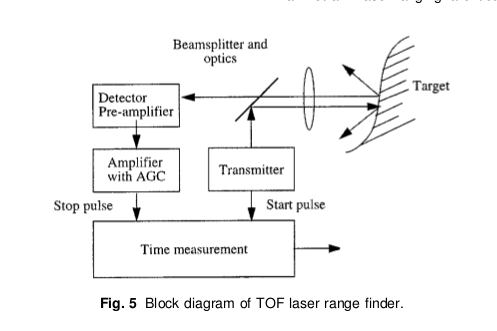
\includegraphics[width=\textwidth]{figures/raycasting/block_diagram.png}
    \caption{\textbf{CHANGE TO TIKZ} Block diagram of \gls{tof} laser range finder\label{fig:lidar_block_diagram}}
\end{figure}
A wide variety of lasers are used depending on the intended measurments range.
In the spacecraft case, laser providing peak energy in the range of \SI{15}{\mega\joule} are often required to measure distance of over \SI{50}{\kilo\meter}~\cite{berry2013}.

The laser range finder is frequently equipped with angle encoders to enable the definition of the position of the measurement point with respect to the sensor. 
Mechanical scanning is performed using a control system which  either move the entire laser range finder or only the measuring beam.
Focal plane scanning is another approach which reduces the mechanical complexity of a mechanical scanning system.
The laser energy illuminates the entire field of view on the surface.
An array of detectors are aranged to view the surface.
Each detector only views a portion of the total field of view and the signals are analyzed in the time domain.
Using this methodology, the system can simulataneously measure distance in multiple directions without any moving parts~\cite{amann2001}.

\subsection{Asteroid Mapping Operations}

Precise relative navigation and landing near asteroids is critically dependent on an accurate knowledge of the shape of the body.
The fine topological structure of the surface is not possible without a spacecraft in the vicinity of the asteroid.
From ground  based measurments, such as radar or optical telescopes, it is only possible to achieve a coarse model of asteroid, such as a triaxial ellipsoid representation~\cite{hudson1994}.
The size and shape of asteroid presents critical information into the thermal and collisional histories and more critically into their internal structure~\cite{cole1998}.

Typical missions spend months after arrival at an asteorid mapping and measuring the surface.
During this mapping phase, which requires upwards of \num{6} months, the spacecraft must maintain a specific trajectory and attitude to ensure best measurements of the surface~\cite{cheng2002,barnouin-jha2008}.
Both the spacecraft orbit and it's attitude is constrained to best satsify the competing requirements of the range measurements, spacecraft power, and Earth based communications.
These measurements are then sent back to Earth, and combined with the spacecraft orbit determination to simulateously estimate the asteroid shape, mass, gravity field, spin state, and spacecraft state.

Look at miller2002 for more detail and discuss that here

% TODO Discuss how the shape of an asteroid is determined in pracice currently
\begin{itemize}
    \item Talk about ground based imaging and citations (radar/optical)
    \item tlak about best knowledge of asteroid before arrival is a ellipsoid model (first mometn)
    \item Talk about sending missions to asteroids with laser altimeters
    \item Months of mapping and ground based OD
\end{itemize}

\subsection{Surface Reconstruction}
One of the main mission objectives for asteroid operations is to generate the three-dimensional shape of an asteroid.
This shape generation is a subset of a larger class of methods called surface reconstruction.
The goal of surface reconstruction is stated as follows: Given a set of sample points \( X\) assumed to lie on /near the surface \( U \), create a surface model \( S \) approximating \( U \).
Surface reconstruction is a well-researched field and widely applied in the industrial and computer vision fields.
The generation of a surface from an object is important in reverse engineering, product design and medical product construction~\cite{amenta2001}.
The surface reconstruction problem is applied in a variety of fields in science and engineering including 3D scanning, surface reconstruction from contours and surface sketching~\cite{hoppe1992}.

Surface reconstruction, or sometimes referred to as 3D scanning, is the generation of accurate models of real world objects.
Surface Reconstruction techniques are frequently used to digitize sculptures/architecture, machine parts, archaeological artifacts, or terrain.
There are a variety of methods to digitize objects, such as laser range finding, mechanical touch probes, or computer vision techniques, i.e. depth from stereo.
From these digitization methods, a large collection, often times on the order of \( 10^6 - 10^9\), of points are generated.
From this \gls{point_cloud}, the goal is to construct a surface representation which is faithful to the original data, and the underlying object of interest.
This process of generating the surface should ideally have the following properties:
\begin{itemize}
    \item Fast - low computational cost
    \item Low memory - storing/operating on large collection of points is frequently memory constrained. Also for use in constrained enviornments
    \item Robustness - Algorithm must be robust to holes, noisy data, varying or low sample density
    \item Accuracy - the method should approximate the shape based on the data rather than interpolating between data points
    \item Features - ability to capture sharp edges or features
\end{itemize}


\subsubsection{3D Scanning}
There are several different approches to acquire shape information of an object.
The computer vision field several approaches exist to determine the shape of an object.
In feature correspondance, landmarks are registered and compared across several different  views of an object. 
The shape of the surface is inferred given the known motion of the camera system~\cite{szeliski2010}.
Another approach is based on the different surface reflectivity of the surface, called shape from shading~\cite{szeliski2010}.

% TODO Mechanical scanning using a probe or laser scanner 
% TODO Range images are generated with distances to the surface. Assume known motion of camera (SLAM) if not known

In 
% TODO Talk about how we construct a mesh given a point cloud
\begin{itemize}
    \item Review surface reconstruction algorithms
    \item Talk about the one that is implemented inside VTK Hoppe papers
    \item 
\end{itemize}

\subsection{Our approach}

Model LIDAR

Simulate measurements

Update shape

Update gravity model

Control based on new estimate of shape


